\documentclass[twoside,openany]{thesis}

\usepackage{xcolor}
\usepackage{hyperref}
\usepackage{graphicx}
\usepackage[backend=biber]{biblatex}

\definecolor{hreflink}{RGB}{150,75,0}
\definecolor{hrefcite}{RGB}{200,0,200}
\definecolor{hrefurl}{RGB}{0,50,200}

\hypersetup{
    colorlinks  = true,
    linkcolor   = hreflink,
    citecolor   = hrefcite,
    urlcolor    = hrefurl
}

\graphicspath{{./images/}}

\addbibresource{references.bib}

\newblock{definition}[num,emph,noterm]
\newblock{theorem}[num,emph,noterm]
\newblock{proof}[nonum,noemph,term]

\title{Design of a document class\linebreak for thesis writing}
\purpose{Thesis uploaded for the good of mankind, in fulfilment\linebreak of the requirements for the degree of}
\degree{Master of \TeX nology}
\subject{Thesis formatting}
\author{\LaTeX\ enthusiast}
\authoraffil{Society of Document Beautifiers\linebreak Indian Institute of \TeX nology}
\mentor{\TeX\ activist}
\mentoraffil{Department Against Word Processors\linebreak Indian Institute of \TeX nology}
\logo{
\includegraphics[scale=0.35]{logo.png}}

\begin{document}

\opening

\maketitle

\front

\chapter{Contents}

\generatetoc

\chapter{List of figures}

\generatelof

\chapter{List of tables}

\generatelot

\main

\chapter{Introduction}\label{ch:Introduction}

This is the user manual for the {\ttfamily thesis} document class, a template designed to simplify the task of thesis writing.
The {\ttfamily thesis} class is largely modelled on the standard {\ttfamily book} class, and produces an output document with a similar structure.
However, the internal workings of the {\ttfamily thesis} class are very different from the {\ttfamily book} class, and were designed to make it fully customisable with minimal effort.
This guide contains usage instructions along with illustrations wherever necessary.
Besides, this document itself was created under the {\ttfamily thesis} class, allowing the reader to see what a document compiled under this class looks like.

The main features implemented in this class have been summarised in the following list.
Each of these features is covered in depth in the upcoming chapters.

\begin{listing}

\item   {\itshape Basic class options}

        Class options can be passed to set the paper and font sizes, choose from among one- and two-sided printing styles, and indicate whether new chapters are allowed to begin on left hand side pages.
        Chapter \ref{ch:Class options} covers this in depth.

\item   {\itshape Book-style structure}

        The output document has a book-like structure.
        It comprises of an opening portion containing the title page, a front portion composed of an abstract, table of contents, list of figures, etc., a main portion which consists of the actual content of the thesis, and a back portion, which contains the bibliography.
        Document structure is the subject of Chapter \ref{ch:Document structure}.

\item   {\itshape Detailed title page}

        The title page contains all details usually found on a thesis cover.
        This includes the project title, the expected degree, names and affiliations of the author and supervisor, and also the university logo.
        Chapter \ref{ch:Title page} describes the procedure for constructing the title page.

\item   {\itshape Automatic tables of contents}

        The table of contents, list of figures, and list of tables are generated automatically by conveniently invoking simple commands, just like in standard \LaTeX\ document classes.
        Chapter \ref{ch:Document contents} covers the commands for doing this.

\clearpage

\item   {\itshape Figure and table environments}

        As discussed in Chapter \ref{ch:Figures and tables}, separate environments are provided to create floating elements such as figures and tables.
        These are identical to the structures implemented in standard document classes.

\item   {\itshape List structures}

        The {\ttfamily thesis} class provides three types of list structures -- bulleted lists, enumerations, and description lists.
        A separate environment is defined for creating each type of listing.
        Detailed information on this can be found in Chapter \ref{ch:Lists and enumerations}.

\item   {\itshape Technical blocks}

        A simple command is provided to define new environments for technical statements such as proofs, definitions, theorems, etc.
        Under standard \LaTeX\ classes, this is done with the help of the {\ttfamily amsthm} package.
        However, the {\ttfamily thesis} class provides this feature as an integral component, eliminating the need for {\ttfamily amsthm}.
        This feature is covered in Chapter \ref{ch:Technical blocks}.

\item   {\itshape Full programmability}

        The {\ttfamily thesis} class was designed by keeping customisation in mind.
        Hence, the class file {\ttfamily thesis.cls} is accompanied by another file {\ttfamily thesis.clo}, which contains a comprehensive list of parameters.
        These parameters can easily be reprogrammed in order to alter the appearance of the output document.
        This interface, covered in Chapter \ref{ch:Modifying class parameters}, offers the user full control over {\itshape all} formatting rules, with very little effort.

\item   {\itshape Hyperlink compatibility}

        Under standard \LaTeX\ classes, automatic hyperlinks (using the {\ttfamily hyperref} package) attached to unnumbered entries in the table of contents point to incorrect locations in the PDF document.
        This behaviour has to be corrected manually by invoking the {\ttfamily\textbackslash phantomsection} command every time an unnumbered element is created.
        However, the {\ttfamily thesis} class makes this correction automatically whenever the {\ttfamily hyperref} package is used, taking this bookkeeping task off the user's shoulders.

\end{listing}

\chapter{Class options}\label{ch:Class options}

A few basic parameters may be passed as options to the {\ttfamily\textbackslash documentclass} command, at the beginning of the source text.
With these options, the user can control the paper and font sizes, select from among one- and two-sided printing styles, and indicate whether new chapters are allowed to open on left hand side pages.
Options are passed along with the {\ttfamily\textbackslash documentclass} command as follows.

{\ttfamily\textbackslash documentclass[<options>]\{thesis\}}

Here, {\ttfamily<options>} is a comma separated list of options to be applied.
This chapter contains a detailed description of all the options defined by the {\ttfamily thesis} class, as well as the concept of default options.

\section{Available options}\label{sec:Available options}

The options defined by the {\ttfamily thesis} class can be grouped into four major categories -- paper size, font size, printing style, and chapter opening options.
The following is a description of the options available under each category.

\subsection{Paper size options}\label{subsec:Paper size options}

One out of three predefined paper sizes may be selected for the document -- A4, letter, and legal.
The corresponding options to choose these respective paper sizes are as follows.

{\ttfamily a4paper,letterpaper,legalpaper}

\subsection{Font size options}\label{subsec:Font size options}

The {\ttfamily thesis} class recognises the three usual font size categories -- 10pt, 11pt, and 12pt.
Each category defines a set of exact font sizes for the standard commands {\ttfamily\textbackslash Huge}, {\ttfamily\textbackslash huge}, ...\ {\ttfamily\textbackslash scriptsize}, {\ttfamily\textbackslash tiny}.
The desired font size category may be selected by passing one of the following options.

{\ttfamily 10pt,11pt,12pt}

\subsection{Printing style options}\label{subsec:Printing style options}

Both one- and two-sided printing styles are possible under the {\ttfamily thesis} class.
In a two-sided printing style, odd-numbered pages appear on the right hand side of the printed book, and even-numbered pages on the left.
In a one-sided document, all pages appear on the right hand side.
The running page headers and footers are defined differently for left, and right hand side pages.
As visible in this very document, odd page numbers are placed on the right side of the page, but even page numbers are placed towards the left.
In one-sided printing, all pages are right hand side pages, and will have identical header and footer formats.
The printing style may be selected by applying one of the following two options.

{\ttfamily oneside,twoside}

\subsection{Chapter opening options}\label{subsec:Chapter opening options}

New chapters may be allowed to either open only on right hand side pages, or on any pages.
Both these schemes are equivalent in one-sided documents.
In a two-sided document however, requiring a new chapter to open on the right hand side means that it can only start on an odd-numbered page, skipping an additional blank page if necessary.
The user may specify their preference by applying any one of the following two options.

{\ttfamily openright,openany}

\section{Default options}\label{sec:Default options}

Options are applied in two successive steps.
First of all, a set of default options is applied, regardless of the options passed by the user.
After this, the user-specified options (if any) are applied, overriding any of the default options if necessary.
The following is the set of default options, which may therefore, be eliminated from the source text.

{\ttfamily a4paper,10pt,oneside,openright}

Thus, a two-sided document with all other parameters set to default, may be created by just passing the {\ttfamily twoside} option alone.

\section{Option summary}\label{sec:Option summary}

The following is a summary of all options defined under the {\ttfamily thesis} class.
Default options have been marked with an asterisk.

\begin{description}[3cm]

\item[{\ttfamily a4paper}*]     A4-sized paper.

\item[{\ttfamily letterpaper}]  Letter-sized paper.

\item[{\ttfamily legalpaper}]   Legal-sized paper.

\item[{\ttfamily 10pt}*]        10pt fonts.

\item[{\ttfamily 11pt}]         11pt fonts.

\item[{\ttfamily 12pt}]         12pt fonts.

\item[{\ttfamily twoside}]      Two-sided printing style.

\item[{\ttfamily oneside}*]     One-sided printing style.

\item[{\ttfamily openright}*]   New chapters must begin on right hand side.

\item[{\ttfamily openany}]      New chapters may begin on any page.

\end{description}

\chapter{Document structure}\label{ch:Document structure}

The {\ttfamily thesis} class implements a hierarchical document structure consisting of {\itshape chapters}, {\itshape sections}, {\itshape subsections}, and {\itshape sub-subsections}.
Additionally, the document is also divided into four major portions -- the {\itshape opening}, {\itshape front}, {\itshape main}, and {\itshape back} portions -- that serve different purposes.
The structure of chapters, and their subsequent sectioning is defined differently for these different portions.

\section{Document portions}\label{sec:Document portions}

The document must begin with the {\itshape opening} portion.
This should be followed by the {\itshape front}, {\itshape main}, and {\itshape back} portions in that order.
The opening portion is meant to contain the title page.
The front portion is composed of all the material that appears before the main content of the thesis begins.
This includes the acknowledgements, abstract, table of contents, list of figures, list of tables, etc.
The main portion contains the actual content of the thesis, divided into multiple chapters and appendices.
The back portion is meant for the bibliography.

The following are the commands for creating the four document portions, along with detailed descriptions of these portions.

\begin{listing}

\item   {\ttfamily\textbackslash opening}

        This command marks the beginning of the opening portion.
        Page headers and footers are not printing in this portion, and page numbering is not performed.
        The title page (see Chapter \ref{ch:Title page}) can only be created in this portion.
        The opening portion is also a good place to put additional pages such as a dedication or a quote, as nothing else shall appear on these pages (like page headers and footers).

\item   {\ttfamily\textbackslash front}

        This command marks the beginning of the front portion.
        It can be executed only if the {\ttfamily\textbackslash opening} command has already been executed.
        Page headers and footers are printed in this portion, and page numbering is performed.
        Page numbers are printed as lower case Roman numerals.
        Chapters created in this portion are unnumbered and represent the abstract, table of contents, etc.

\item   {\ttfamily\textbackslash main}

        This command marks the beginning of the main portion.
        It can be executed only if the {\ttfamily\textbackslash front} command has already been executed.
        Page headers and footers are printed in this portion.
        Page numbering is restarted from 1, and page numbers are printed in the ordinary Arabic format.
        Chapters created in this portion are numbered and represent ordinary chapters as well as appendices that constitute the main content of the thesis.

\item   {\ttfamily\textbackslash back}

        This command marks the beginning of the back portion.
        It can be executed only if the {\ttfamily\textbackslash main} command has already been executed.
        Page headers and footers are printed in this portion.
        Page numbering continues from the main portion into this portion.
        Chapters created in this portion are unnumbered.
        The back portion will usually consist of only one chapter, and that is used to represent the bibliography.

\end{listing}

Thus, the overall structure of the source text should be as follows.

{\ttfamily
    \textbackslash begin\{document\}\linebreak
    \textbackslash opening\linebreak
        \null\quad<contents of opening portion>\linebreak
    \textbackslash front\linebreak
        \null\quad<contents of front portion>\linebreak
    \textbackslash main\linebreak
        \null\quad<contents of main portion>\linebreak
    \textbackslash back\linebreak
        \null\quad<contents of back portion>\linebreak
    \textbackslash end\{document\}
}

\section{Chapters}\label{sec:Chapters}

Chapters are the primary structures for document sectioning in the {\ttfamily thesis} class.
A chapter can be created with the {\ttfamily\textbackslash chapter} command, as follows.

{\ttfamily\textbackslash chapter\{<chapter-name>\}}

Here, {\ttfamily<chapter-name>} is the name of the chapter being created.
Depending on the document portion in which the above command is executed, different outcomes can be observe, as elaborated below.

\begin{listing}

\item   {\itshape Opening portion}

        A compilation failure occurs.
        Chapter creation is not allowed in the opening portion.

\item   {\itshape Front portion}

        An unnumbered chapter is created.
        The current page is skipped if not blank, and an unnumbered chapter heading containing the chapter name is created on the new page.
        If the {\ttfamily twoside} and {\ttfamily openright} class options were applied, then an additional page may be skipped to ensure that the new chapter begins on an odd-numbered page.
        An entry for the new chapter is added to the table of contents (see Chapter \ref{ch:Document contents}).
        Page headers are updated to indicate the current chapter.
        The front portion will usually comprise chapters like {\ttfamily\textbackslash chapter\{Abstract\}}, {\ttfamily\textbackslash chapter\{Contents\}}, {\ttfamily\textbackslash chapter\{List of figures\}}, {\ttfamily\textbackslash chapter\{List of tables\}}, etc.

\item   {\itshape Main portion}

        A numbered chapter is created.
        The current page is skipped if not blank, and a chapter heading containing the chapter name and number is created on the new page.
        If the {\ttfamily twoside} and {\ttfamily openright} class options were applied, then an additional page may be skipped to ensure that the new chapter begins on an odd-numbered page.
        An entry for the new chapter is added to the table of contents.
        Page headers are updated to indicate the current chapter.
        In the main portion, one of two modes -- {\itshape chapter} and {\itshape appendix} -- may be active.
        Chapter numbers are printed in Arabic format in chapter mode, and alphabetically in appendix mode.
        The mode can be switched by using the {\ttfamily\textbackslash appendix} command, described further below.

\item   {\itshape Back portion}

        An unnumbered chapter is created.
        The process is identical to that of chapter creation in the front portion.
        The back portion will usually consist of a single chapter, namely {\ttfamily\textbackslash chapter\{Bibliography\}}.

\end{listing}

As mentioned above, two modes -- {\itshape chapter} and {\itshape appendix} -- are possible in the main portion.
Upon starting the main portion with the {\ttfamily\textbackslash main} command, the chapter mode is automatically activated.
The command {\ttfamily\textbackslash appendix} may be invoked at any point in the main portion, to switch to appendix mode.
This command can be run only once.
Also, it is not possible to switch back from appendix to chapter mode (should this ever become necessary, you should realise that you have designed your document badly).

To sum up, the structure of the main portion in the source text should be similar to the following snippet.

{\ttfamily
    \textbackslash main\linebreak
    \textbackslash chapter\{<first chapter name>\}\linebreak
        \null\quad<first chapter content>\linebreak
    \textbackslash chapter\{<second chapter name>\}\linebreak
        \null\quad<second chapter content>\linebreak
    \textbackslash appendix\linebreak
    \textbackslash chapter\{<first appendix name>\}\linebreak
        \null\quad<first appendix content>\linebreak
    \textbackslash chapter\{<second appendix name>\}\linebreak
        \null\quad<second appendix content>
}

\section{Further sectioning}\label{sec:Further sectioning}

The {\ttfamily thesis} class offers three hierarchical levels of sectioning within a chapter.
These are achieved by invoking the {\ttfamily\textbackslash section}, {\ttfamily\textbackslash subsection}, and {\ttfamily\textbackslash subsubsection} commands.
The syntax for each of these commands is similar to that of the {\ttfamily\textbackslash chapter} command.

{\ttfamily
\textbackslash section\{<section name>\}\linebreak
\textbackslash subsection\{<subsection name>\}\linebreak
\textbackslash subsubsection\{<sub-subsection name>\}
}

The above commands create a section, subsection, or sub-subsection header, and add a corresponding entry to the table of contents.
The section, subsection, or sub-subsection thus created is numbered if created within a numbered chapter, and unnumbered if created within an unnumbered chapter.

It is only possible to proceed in steps of one hierarchical level at a time.
This means that a section can only be created within a chapter, a subsection within a section, and so on.
Not doing so will result in an ``insufficient sectioning depth'' error upon compilation (in standard \LaTeX\ document classes, compilation succeeds but leads to absurd numbering).

\section{Note on undefined commands}\label{sec:Note on undefined commands}

The {\ttfamily thesis} class does not define the familiar starred commands {\ttfamily\textbackslash chapter*}, {\ttfamily\textbackslash section*}, etc.
Also, the commands {\ttfamily\textbackslash part}, {\ttfamily\textbackslash paragraph}, and {\ttfamily\textbackslash subparagraph} are not defined, at least as of now.

\chapter{Title page}\label{ch:Title page}

The {\ttfamily thesis} class features a detailed title page which contains the project title, expected degree, names and affiliations of the author and supervisor, and the university logo.
Under this document class, the title page can only be created in the opening portion (see Section \ref{sec:Document portions}).

\section{Title page parameters}\label{sec:Title page parameters}

The procedure to create a title page is identical to that of standard \LaTeX\ document classes.
Values must be defined for a set of parameters, which are then put together by the {\ttfamily\textbackslash maketitle} command to form the title page.

The following is a list of commands that set values for the different parameters required to generate the title page.
It is necessary to run each of the following commands once before invoking {\ttfamily\textbackslash maketitle}.
The following commands are usually placed in the preamble of the source text, but this is not a strict rule to follow.

\begin{listing}

\item   {\ttfamily\textbackslash title\{<project-title>\}}

        Sets the thesis project title to {\ttfamily<project-title>}.
        The project title appears at the top of the title page.

\item   {\ttfamily\textbackslash purpose\{<submission-purpose>\}}

        Sets {\ttfamily<submission-purpose>} as the phrase indicating the purpose of submission of the thesis.
        This will usually be a phrase like ``Thesis submitted in partial fulfilment of the requirements for the degree of''.
        Following this phrase, the expected degree title (see next command) appears right below.
        The degree title should not be included in the phrase {\ttfamily<submission-purpose>}.

\item   {\ttfamily\textbackslash degree\{<expected-degree>\}}

        Sets the expected degree title to {\ttfamily<expected-degree>}.
        The degree title must not include the academic field in which it shall be awarded.
        For instance, ``Bachelor of Science'' or ``Doctor of Philosophy'' are appropriate values for {\ttfamily<expected-degree>}, but ``Bachelor of Science in Physics'' is not.
        The academic field appears on a separate line and is specified by the next command in this list.

\item   {\ttfamily\textbackslash subject\{<academic-field>\}}

        Sets the academic field in which the degree shall be awarded, to {\ttfamily<academic-field>}.
        For example, ``Physics'', ``Aerospace engineering'', etc.\ are appropriate values.
        Together with the degree title, this results in a phrase like ``Bachelor of Science in Physics'' split over multiple lines.

\item   {\ttfamily\textbackslash author\{<author-name>\}}

        Sets the name of the author to {\ttfamily<author-name>}.

\item   {\ttfamily\textbackslash authoraffil\{<author-affiliation>\}}

        Sets the author's affiliation to {\ttfamily<author-affiliation>}.
        For instance, the name of the author's department in the university could be specified as {\ttfamily<author-affiliation>}.

\item   {\ttfamily\textbackslash mentor\{<mentor-name>\}}

        Sets the name of the project supervisor to {\ttfamily<mentor-name>}.

\item   {\ttfamily\textbackslash mentoraffil\{<mentor-affiliation>\}}

        Sets the project supervisor's affiliation to {\ttfamily<mentor-affiliation>}.
        For instance, the name of the project supervisor's department in the university could be specified as {\ttfamily<mentor-affiliation>}.

\item   {\ttfamily\textbackslash logo\{<university-logo>\}}

        Sets the command to generate the university logo, to {\ttfamily<university-logo>}.
        Thus, {\ttfamily<university-logo>} will itself be a command, usually containing an invocation of {\ttfamily\textbackslash includegraphics}.

\end{listing}

\section{Generating the title}\label{sec:Generating the title}

Once each of the commands listed in Section \ref{sec:Title page parameters} has been run, the title page can be created by simply executing the {\ttfamily\textbackslash maketitle} command.
However, it must be kept in mind that {\ttfamily\textbackslash maketitle} can only be called in the opening portion (see Section \ref{sec:Document portions}) of the document.
Thus, the part of the source text that generates the title page must resemble the following snippet.

{\ttfamily
    \textbackslash title\{<project-title>\}\linebreak
    \textbackslash purpose\{<submission-purpose>\}\linebreak
    \textbackslash degree\{<expected-degree>\}\linebreak
    \textbackslash subject\{<academic-field>\}\linebreak
    \textbackslash author\{<author-name>\}\linebreak
    \textbackslash authoraffil\{<author-affiliation>\}\linebreak
    \textbackslash mentor\{<mentor-name>\}\linebreak
    \textbackslash mentoraffil\{<mentor-affiliation>\}\linebreak
    \textbackslash logo\{<university-logo>\}\linebreak
    \linebreak
    \textbackslash begin\{document\}\linebreak
    \textbackslash opening\linebreak
        \null\quad\textbackslash maketitle\linebreak
    \textbackslash front\linebreak
        \null\quad\textbackslash<front-matter>\linebreak
    \textbackslash main\linebreak
        \null\quad\textbackslash<main-matter>\linebreak
    \textbackslash back\linebreak
        \null\quad\textbackslash<back-matter>\linebreak
    \textbackslash end\{document\}\linebreak
}

\chapter{Document contents}\label{ch:Document contents}

The {\ttfamily thesis} class provides commands to generate three basic listings of contents -- the table of contents, list of figures, and the list of tables.
The usual place to create these lists is the front portion (see Section \ref{sec:Document portions}) of the document.
The corresponding commands are as follows.

\begin{listing}

\item   {\ttfamily\textbackslash generatetoc}

        Lists out the {\itshape table of contents}.
        This includes all document sectioning structures described in Chapter \ref{ch:Document structure} -- chapters, sections, subsections, and sub-subsections.
        Numbered as well as unnumbered elements are listed out.

\item   {\ttfamily\textbackslash generatelof}

        Lists out the {\itshape list of figures}.
        This includes all figures created using the {\ttfamily figure} environment.
        The {\ttfamily figure} environment is discussed in detail in Chapter \ref{ch:Figures and tables}.

\item   {\ttfamily\textbackslash generatelot}

        Lists out the {\itshape list of tables}.
        This includes all tables created using the {\ttfamily table} environment.
        The {\ttfamily table} environment is discussed in detail in Chapter \ref{ch:Figures and tables}.

\end{listing}

While these commands list out their corresponding document contents, they do not first navigate to a new page or create a heading.
In order to create the necessary headings, and start each of these lists on new pages, the above commands must be invoked within separate chapters.
Thus, an appropriate method to list out the document contents would be as follows.

{\ttfamily
    \textbackslash front\linebreak
    <any other content, such as abstract, acknowledgements, etc.>\linebreak
    \textbackslash chapter\{Contents\}\linebreak
        \null\quad\textbackslash generatetoc\linebreak
    \textbackslash chapter\{List of figures\}\linebreak
        \null\quad\textbackslash generatelof\linebreak
    \textbackslash chapter\{List of tables\}\linebreak
        \null\quad\textbackslash generatelot\linebreak
}

\chapter{Figures and tables}\label{ch:Figures and tables}

Figures and tables are created as {\itshape floating} structures (elements that treated separately from the main text in the document).
We first discuss the basics of floating structures in Section \ref{sec:Floating elements}.
Following this, Sections \ref{sec:Figures} and \ref{sec:Tables} cover the processes of creating figures and tables respectively.

\section{Floating elements}\label{sec:Floating elements}

Floating elements are structures that will never be split over multiple pages.
Also, they are not part of the regular stream of text, and are placed in a separately allocated part of the page.
The compiler may choose from among various different positions to place a floating element -- top of page, bottom of page, approximately where it appears in the source text, or on a separate special page for floats only.
Each of these locations is represented by a corresponding {\itshape placement specifier} (see Table \ref{tab:Float placement specifiers}).
The user may optionally pass one or more placement specifier while creating a floating element.
This instructs the \LaTeX\ compiler to choose from only those locations, while placing the floating element in question.

Each floating structure is implemented as a separate numbered environment (thus, the {\ttfamily thesis} class recognises two environments -- {\ttfamily figure} and {\ttfamily table}).
Every floating element has a {\itshape caption} that indicates this number, and also contains a short description written by the user.
Also, floating elements can be created only within numbered chapters, as their numbering includes the chapter number.

\begin{table}
    \begin{center}
        \begin{tabular}{|l|l|}
            \hline
            \multicolumn{1}{|c|}{Specifier} & \multicolumn{1}{|c|}{Placement position}\\
            \hline
            \hline
            {\ttfamily h} & Place float approximately {\itshape here} (same point it occurs in source text).\\
            {\ttfamily t} & Place float at the {\itshape top} of the page.\\
            {\ttfamily b} & Place float at the {\itshape bottom} of the page.\\
            {\ttfamily p} & Create a special {\itshape page} just for floats and place float there.\\
            \hline
        \end{tabular}
    \end{center}
    \caption[Floating structure placement specifiers]{
        List of placement specifiers that can optionally be passed while creating a floating structure.
        The default set of specifiers passed is {\ttfamily tbp}.
    }
    \label{tab:Float placement specifiers}
\end{table}

The code to generate a floating element of any kind is as follows.

{\ttfamily
    \textbackslash begin\{<envname>\}[<placement>]\linebreak
        \null\quad<content>\linebreak
        \null\quad\textbackslash caption[<captshort>]\{<captlong>\}\linebreak
        \null\quad\textbackslash label\{<labname>\}\linebreak
    \textbackslash end\{<envname>\}
}

Here, {\ttfamily<envname>} is the name of the floating environment (in the {\ttfamily thesis} class, this will be either {\ttfamily figure} or {\ttfamily table}).
The {\ttfamily<placement>} argument represents the optional placement specifiers.
If left unspecified, the default placement specifiers {\ttfamily tbp} are passed.
The code to generate the actual content of the floating element (the image or table) must replace {\ttfamily<content>}.
Two kinds of captions can be specified.
A long caption {\ttfamily<captlong>} is what appears along with the floating element as the actual caption, and a short caption {\ttfamily<captshort>} goes into the list of figures or list of tables.
A label {\ttfamily<labname>} can be attached for use with the {\ttfamily\textbackslash ref} command.

\section{Figures}\label{sec:Figures}

Figures are created using the floating environment {\ttfamily figure}.
The image can be created using the {\ttfamily\textbackslash includegraphics} command from the {\ttfamily graphicx} package.
Detailed information about the {\ttfamily graphicx} package can be found in its \href{http://packages.oth-regensburg.de/ctan/macros/latex/required/graphics/grfguide.pdf}{official documentation}.

For example, the following code was executed to generate Figures \ref{fig:examplefigure1} and \ref{fig:examplefigure2}.

{\ttfamily
    \textbackslash begin\{figure\}[p]\linebreak
        \null\quad\textbackslash begin\{center\}\linebreak
            \null\quad\quad\textbackslash includegraphics[scale=0.075]\{examplefigure1.jpg\}\linebreak
        \null\quad\textbackslash end\{center\}\linebreak
        \null\quad\textbackslash caption[Short title for example figure 1]\{\linebreak
            \null\quad\quad This is a detailed description of example figure 1.\linebreak
            \null\quad\quad It appears along with the figure, as a paragraph in the caption.\linebreak
            \null\quad\quad The short title for this figure appears in the list of figures.\linebreak
        \null\quad\}\linebreak
        \null\quad\textbackslash label\{fig:examplefigure1\}\linebreak
    \textbackslash end\{figure\}
}

{\ttfamily
    \textbackslash begin\{figure\}[p]\linebreak
        \null\quad\textbackslash begin\{center\}\linebreak
            \null\quad\quad\textbackslash includegraphics[scale=0.3]\{examplefigure2.jpg\}\linebreak
        \null\quad\textbackslash end\{center\}\linebreak
        \null\quad\textbackslash caption[Short title for example figure 2]\{\linebreak
            \null\quad\quad This is a detailed description of example figure 2.\linebreak
            \null\quad\quad It appears along with the figure, as a paragraph in the caption.\linebreak
            \null\quad\quad The short title for this figure appears in the list of figures.\linebreak
        \null\quad\}\linebreak
        \null\quad\textbackslash label\{fig:examplefigure2\}\linebreak
    \textbackslash end\{figure\}
}

\clearpage

\section{Tables}\label{sec:Tables}

Tables are created using the floating environment {\ttfamily table}.
The tabular arrangement can be created using the {\ttfamily tabular} environment.
Detailed information about the {\ttfamily tabular} environment can be found on \href{https://en.wikibooks.org/wiki/LaTeX/Tables}{wikibooks}.

For example, the following code was executed to generate Tables \ref{tab:exampletable1} and \ref{tab:exampletable2}.

{\ttfamily
    \textbackslash begin\{table\}[p]\linebreak
        \null\quad\textbackslash begin\{center\}\linebreak
            \null\quad\quad\textbackslash begin\{tabular\}\{|c|c|c|\}\linebreak
                \null\quad\quad\textbackslash hline\linebreak
                \null\quad\quad\$P\_\{11\}\$ \& \$P\_\{12\}\$ \& \$P\_\{13\}\$\textbackslash\textbackslash\linebreak
                \null\quad\quad\textbackslash hline\linebreak
                \null\quad\quad\$P\_\{21\}\$ \& \$P\_\{22\}\$ \& \$P\_\{23\}\$\textbackslash\textbackslash\linebreak
                \null\quad\quad\textbackslash hline\linebreak
            \null\quad\quad\textbackslash end\{tabular\}\linebreak
        \null\quad\textbackslash end\{center\}\linebreak
        \null\quad\textbackslash caption[Short title for example table 1]\{\linebreak
            \null\quad\quad This is a detailed description of example table 1.\linebreak
            \null\quad\quad It appears along with the table, as a paragraph in the caption.\linebreak
            \null\quad\quad The short title for this table appears in the list of tables.\linebreak
        \null\quad\}\linebreak
        \null\quad\textbackslash label\{tab:exampletable1\}\linebreak
    \textbackslash end\{table\}
}

{\ttfamily
    \textbackslash begin\{table\}[p]\linebreak
        \null\quad\textbackslash begin\{center\}\linebreak
            \null\quad\quad\textbackslash begin\{tabular\}\{|c|c|c|\}\linebreak
                \null\quad\quad\textbackslash hline\linebreak
                \null\quad\quad\$Q\_\{11\}\$ \& \$Q\_\{12\}\$ \& \$Q\_\{13\}\$\textbackslash\textbackslash\linebreak
                \null\quad\quad\textbackslash hline\linebreak
                \null\quad\quad\$Q\_\{21\}\$ \& \$Q\_\{22\}\$ \& \$Q\_\{23\}\$\textbackslash\textbackslash\linebreak
                \null\quad\quad\textbackslash hline\linebreak
            \null\quad\quad\textbackslash end\{tabular\}\linebreak
        \null\quad\textbackslash end\{center\}\linebreak
        \null\quad\textbackslash caption[Short title for example table 2]\{\linebreak
            \null\quad\quad This is a detailed description of example table 2.\linebreak
            \null\quad\quad It appears along with the table, as a paragraph in the caption.\linebreak
            \null\quad\quad The short title for this table appears in the list of tables.\linebreak
        \null\quad\}\linebreak
        \null\quad\textbackslash label\{tab:exampletable2\}\linebreak
    \textbackslash end\{table\}
}

\begin{figure}[p]
    \begin{center}
        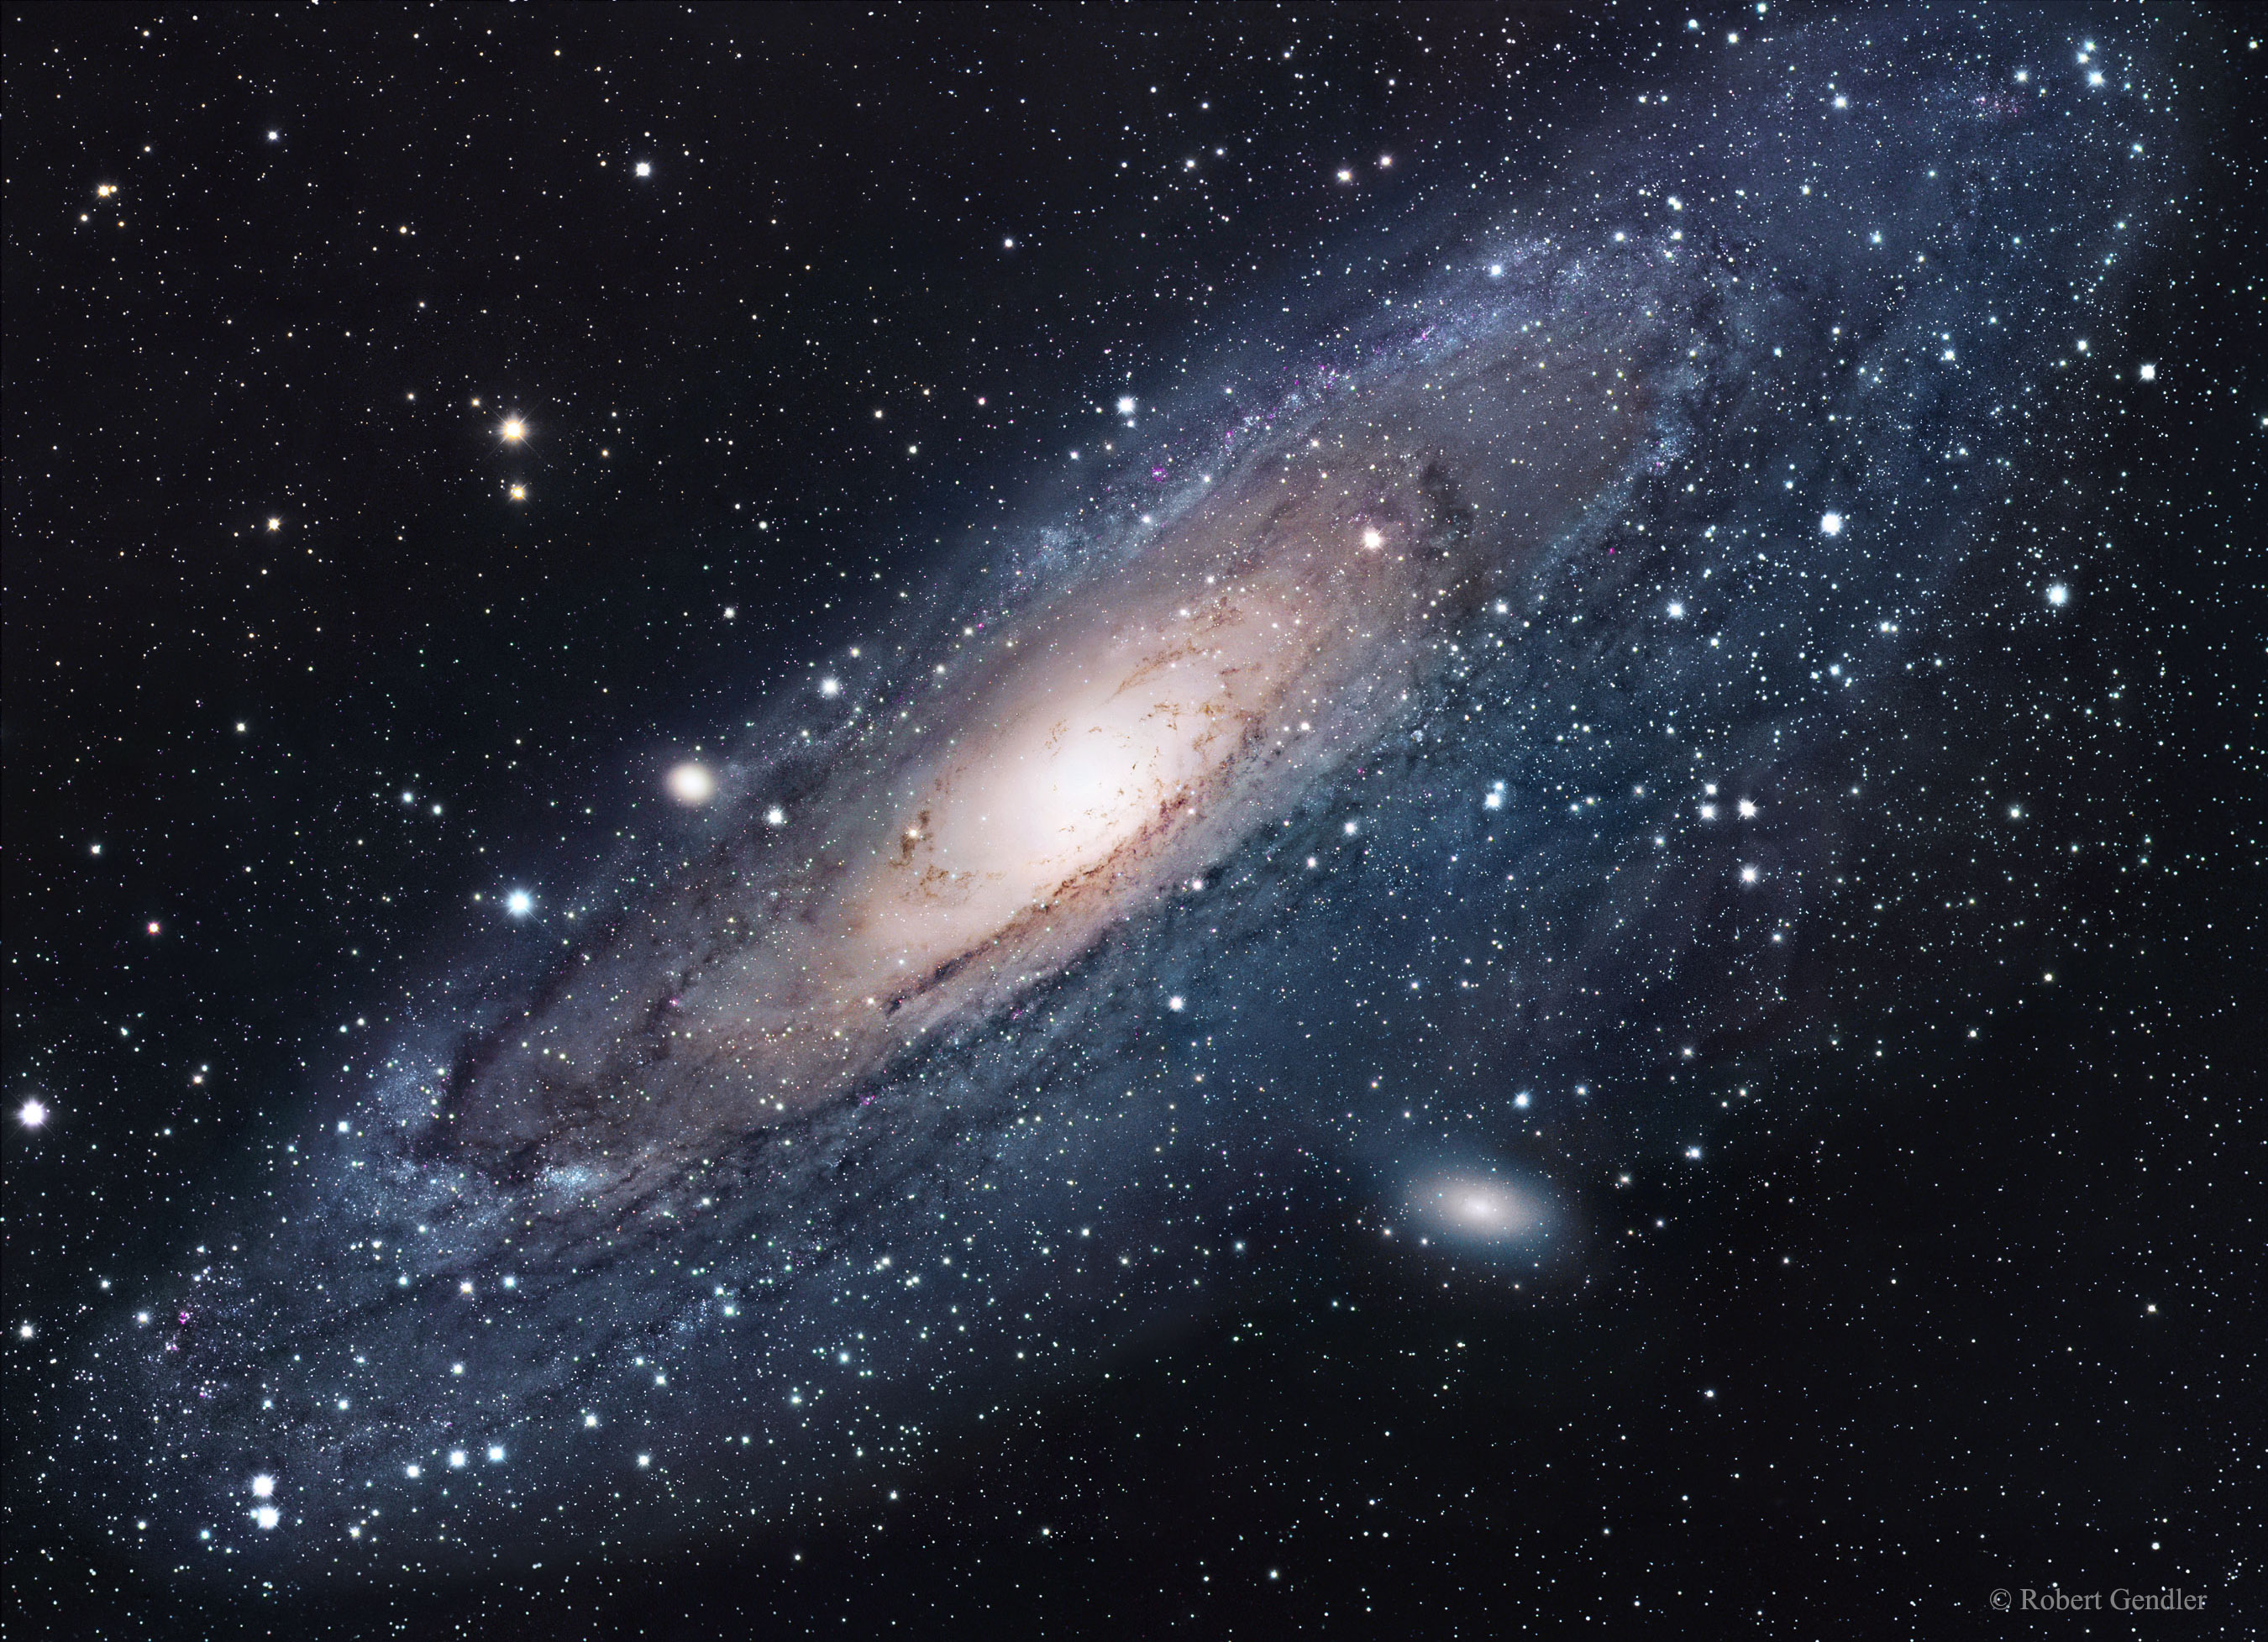
\includegraphics[scale=0.075]{examplefigure1.jpg}
    \end{center}
    \caption[Short title for example figure 1]{
        This is a detailed description of example figure 1.
        It appears along with the figure, as a paragraph in the caption.
        The short title for this figure appears in the list of figures.
    }
    \label{fig:examplefigure1}
\end{figure}

\begin{figure}[p]
    \begin{center}
        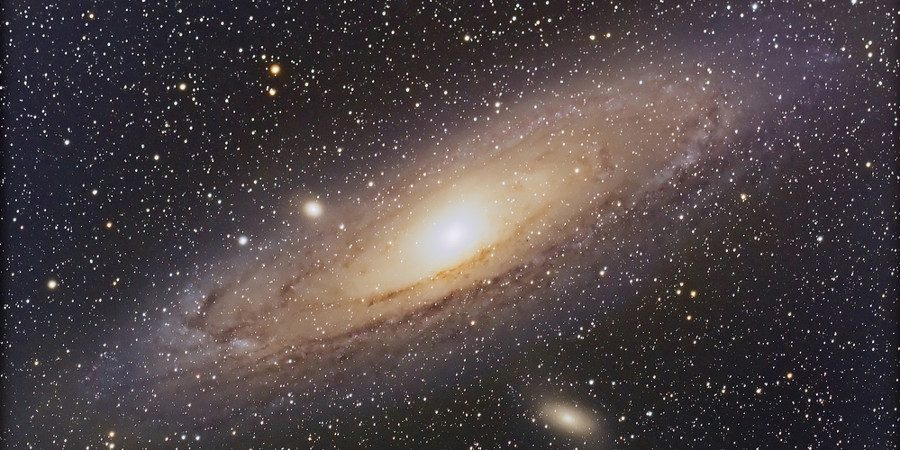
\includegraphics[scale=0.2]{examplefigure2.jpg}
    \end{center}
    \caption[Short title for example figure 2]{
        This is a detailed description of example figure 2.
        It appears along with the figure, as a paragraph in the caption.
        The short title for this figure appears in the list of figures.
    }
    \label{fig:examplefigure2}
\end{figure}

\begin{table}[p]
    \begin{center}
        \begin{tabular}{|c|c|c|}
            \hline
            $P_{11}$ & $P_{12}$ & $P_{13}$\\
            \hline
            $P_{21}$ & $P_{22}$ & $P_{23}$\\
            \hline
        \end{tabular}
    \end{center}
    \caption[Short title for example table 1]{
        This is a detailed description of example table 1.
        It appears along with the table, as a paragraph in the caption.
        The short title for this table appears in the list of tables.
    }
    \label{tab:exampletable1}
\end{table}

\begin{table}[p]
    \begin{center}
        \begin{tabular}{|c|c|c|}
            \hline
            $Q_{11}$ & $Q_{12}$ & $Q_{13}$\\
            \hline
            $Q_{21}$ & $Q_{22}$ & $Q_{23}$\\
            \hline
        \end{tabular}
    \end{center}
    \caption[Short title for example table 2]{
        This is a detailed description of example table 2.
        It appears along with the table, as a paragraph in the caption.
        The short title for this table appears in the list of tables.
    }
    \label{tab:exampletable2}
\end{table}

\chapter{Lists and enumerations}\label{ch:Lists and enumerations}

Three different types of lists can be created under the {\ttfamily thesis} document class -- bulleted, numbered, and description lists.
Each such list structure is implemented as a different environment.
The environments that correspond to bulleted, numbered, and description lists respectively are {\ttfamily listing}, {\ttfamily enumeration}, and {\ttfamily description}.

\section{Basic syntax}\label{sec:Basic syntax}

A list consists of multiple entries packed into one of the three list structures mentioned above.
List entries are created by executing the {\ttfamily\textbackslash item} command, followed by the corresponding text.
In the output document, each list entry starts with a left-aligned label (which can be a bullet, a number, or a description title).
A fixed margin is reserved on the left side for the label.
The textual content appears after the label, and is formatted into paragraphs.
The following syntax applies for creating any of the three kinds of lists.
This snippet shows two entries, but there can be any number of them in general.

{\ttfamily
    \textbackslash begin\{<envname>\}[<labwidth>]\linebreak
    \textbackslash item[<label1>]\quad<Text1>\linebreak
    \textbackslash item[<label2>]\quad<Text2>\linebreak
    \textbackslash end\{<envname>\}
}

Here, {\ttfamily<envname>} must be either {\ttfamily listing}, {\ttfamily enumeration}, or {\ttfamily description}.
The optional label width {\ttfamily<labwidth>} is the margin reserved for entry labels.
If unspecified, a default label width is applied.
The individual labels for the two entries in the above snippet are {\ttfamily<label1>} and {\ttfamily<label2>}, and are also optional.
For bulleted lists and enumerations, it is generally a good idea to leave them unspecified, and let the default labels appear.
In description lists however, these are meant to be specified by the user as they represent description titles.
The texts corresponding to the two entries in the above example are {\ttfamily<Text1>} and {\ttfamily<Text2>}, and may each contain multiple paragraphs.

List entries may themselves contain lists too, resulting in a nested list structure.
Bulleted and numbered lists (created with the {\ttfamily listing} and {\ttfamily enumeration} environments) can be nested only up to 4 levels.
Description lists on the other hand, can be nested indefinitely.

\section{List examples}\label{sec:List examples}

The following examples illustrate the creation of all three kinds of lists.
Notice the change in label format at different levels in the bulleted, and numbered lists.

\subsection{Bulleted list}\label{subsec:Bulleted list}

{\ttfamily
    \textbackslash begin\{listing\}\linebreak
    \textbackslash item\ \ \ Item 1\linebreak
    \null\ \ \ \ \ \ \ \ \textbackslash begin\{listing\}\linebreak
    \null\ \ \ \ \ \ \ \ \textbackslash item\ \ \ Item 1.1\linebreak
    \null\ \ \ \ \ \ \ \ \textbackslash item\ \ \ Item 1.2\linebreak
    \null\ \ \ \ \ \ \ \ \textbackslash end\{listing\}\linebreak
    \textbackslash item\ \ \ Item 2\linebreak
    \null\ \ \ \ \ \ \ \ \textbackslash begin\{listing\}\linebreak
    \null\ \ \ \ \ \ \ \ \textbackslash item\ \ \ Item 2.1\linebreak
    \null\ \ \ \ \ \ \ \ \textbackslash item\ \ \ Item 2.2\linebreak
    \null\ \ \ \ \ \ \ \ \textbackslash end\{listing\}\linebreak
    \textbackslash end\{listing\}
}

\begin{listing}
\item   Item 1
        \begin{listing}
        \item   Item 1.1
        \item   Item 1.2
        \end{listing}
\item   Item 2
        \begin{listing}
        \item   Item 2.1
        \item   Item 2.2
        \end{listing}
\end{listing}

\subsection{Numbered list}\label{subsec:Numbered list}

{\ttfamily
    \textbackslash begin\{enumeration\}\linebreak
    \textbackslash item\ \ \ Item 1\linebreak
    \null\ \ \ \ \ \ \ \ \textbackslash begin\{enumeration\}\linebreak
    \null\ \ \ \ \ \ \ \ \textbackslash item\ \ \ Item 1.1\linebreak
    \null\ \ \ \ \ \ \ \ \textbackslash item\ \ \ Item 1.2\linebreak
    \null\ \ \ \ \ \ \ \ \textbackslash end\{enumeration\}\linebreak
    \textbackslash item\ \ \ Item 2\linebreak
    \null\ \ \ \ \ \ \ \ \textbackslash begin\{enumeration\}\linebreak
    \null\ \ \ \ \ \ \ \ \textbackslash item\ \ \ Item 2.1\linebreak
    \null\ \ \ \ \ \ \ \ \textbackslash item\ \ \ Item 2.2\linebreak
    \null\ \ \ \ \ \ \ \ \textbackslash end\{enumeration\}\linebreak
    \textbackslash end\{enumeration\}
}

\begin{enumeration}
\item   Item 1
        \begin{enumeration}
        \item   Item 1.1
        \item   Item 1.2
        \end{enumeration}
\item   Item 2
        \begin{enumeration}
        \item   Item 2.1
        \item   Item 2.2
        \end{enumeration}
\end{enumeration}

\clearpage

\subsection{Description list}\label{subsec:Description list}

{\ttfamily
    \textbackslash begin\{description\}[1.5cm]\linebreak
    \textbackslash item[Item 1]\ \ \ Description of item 1\linebreak
    \textbackslash item[Item 2]\ \ \ Description of item 2\linebreak
    \textbackslash item[Item 3]\ \ \ Description of item 3\linebreak
    \textbackslash end\{description\}
}

\begin{description}[1.5cm]
\item[Item 1]   Description of item 1
\item[Item 2]   Description of item 2
\item[Item 3]   Description of item 3
\end{description}

\chapter{Technical blocks}\label{ch:Technical blocks}

Technical blocks are a special feature implemented in the {\ttfamily thesis} class, for formatting technical statements like theorems, definitions, proofs, etc.
Under the standard \LaTeX\ document classes, the {\ttfamily amsthm} package provides this functionality.
However, this package is not required while working with the {\ttfamily thesis} class.

\section{Block environments}\label{sec:Block environments}

We use the term {\itshape block} to represent any chunk of text that constitutes a theorem, proof, definition, or any other type of technical statement.
Each such type of technical statement must be associated with a separate {\itshape block environment}.
For example, the user may define three environments -- {\ttfamily theorem}, {\ttfamily proof}, and {\ttfamily definition} -- to create a theorem block, proof block, or definition block.
In order to easily define such block environments, the {\ttfamily thesis} class provides a special command {\ttfamily\textbackslash newblock}, with the following syntax.

{\ttfamily\textbackslash newblock\{<envname>\}[<flags>]}

Here, {\ttfamily<envname>} is the name of the new environment being defined.
It is also the heading text for the newly defined block.
Whenever a new block is created with the command {\ttfamily\textbackslash begin\{<envname>\}}, the word {\ttfamily<envname>} (with its first alphabet capitalised) appears as a heading.
If the block is numbered (which is controlled by the {\ttfamily<flags>} argument), the heading also contains the block number.
The argument {\ttfamily<flags>} is a comma separated list of three options, one from each of the following three sets.
The order in which these options are listed does not matter.

\begin{listing}

\item   {\ttfamily num, nonum}

        The {\ttfamily num} option makes {\ttfamily<envname>} a numbered environment, and {\ttfamily nonum} makes it unnumbered.

\item   {\ttfamily emph, noemph}

        The {\ttfamily emph} option italicises the text within the block, and {\ttfamily noemph} leaves it upright.

\item   {\ttfamily term, noterm}

        The {\ttfamily term} option prints a Q.E.D.\ symbol at the end of the block, and {\ttfamily noterm} avoids it.

\end{listing}

\section{Examples of blocks}\label{sec:Examples of blocks}

In the following example, three block environments are defined to create theorems, definitions, and proofs.
The {\ttfamily\textbackslash newblock} command is invoked in the preamble of the source text.

{\ttfamily
    \textbackslash newblock\{definition\}[num,emph,noterm]\linebreak
    \textbackslash newblock\{theorem\}[num,emph,noterm]\linebreak
    \textbackslash newblock\{proof\}[nonum,noemph,term]
}

Having defined the three environments, they can be used inside the document, to create theorem, proof, and definition blocks.
The following snippet creates a definition block, and two theorem blocks accompanied with corresponding proof blocks, as shown below it.

{\ttfamily
    \textbackslash begin\{definition\}\linebreak
    This is a simple definition.\linebreak
    It appears with a numbered heading of its own.\linebreak
    The definition text is italicised.\linebreak
    \textbackslash end\{definition\}\linebreak
    \linebreak
    \textbackslash begin\{theorem\}\textbackslash label\{thm:theorem1\}\linebreak
    This is a simple theorem.\linebreak
    Its format is similar to that of a definition.\linebreak
    \textbackslash end\{theorem\}\linebreak
    \linebreak
    \textbackslash begin\{proof\}\linebreak
    This is the proof of Theorem \textbackslash ref\{thm:theorem1\}.\linebreak
    It appears with an unnumbered heading.\linebreak
    The proof text is not italicised.\linebreak
    At the end of this proof, you shall find a Q.E.D.\textbackslash \ symbol.\linebreak
    \textbackslash end\{proof\}\linebreak
    \linebreak
    \textbackslash begin\{theorem\}\textbackslash label\{thm:theorem2\}\linebreak
    This is another simple theorem.\linebreak
    Its format is similar to that of a definition.\linebreak
    \textbackslash end\{theorem\}\linebreak
    \linebreak
    \textbackslash begin\{proof\}\linebreak
    This is the proof of Theorem \textbackslash ref\{thm:theorem2\}.\linebreak
    It appears with an unnumbered heading.\linebreak
    The proof text is not italicised.\linebreak
    At the end of this proof, you shall find a Q.E.D.\textbackslash \ symbol.\linebreak
    \textbackslash end\{proof\}\linebreak
}

\begin{definition}
This is a simple definition.
It appears with a numbered heading of its own.
The definition text is italicised.
\end{definition}

\begin{theorem}\label{thm:theorem1}
This is a simple theorem.
Its format is similar to that of a definition.
\end{theorem}

\begin{proof}
This is the proof of Theorem \ref{thm:theorem1}.
It appears with an unnumbered heading.
The proof text is not italicised.
At the end of this proof, you shall find a Q.E.D.\ symbol.
\end{proof}

\begin{theorem}\label{thm:theorem2}
This is another simple theorem.
Its format is similar to that of a definition.
\end{theorem}

\begin{proof}
This is the proof of Theorem \ref{thm:theorem2}.
It appears with an unnumbered heading.
The proof text is not italicised.
At the end of this proof, you shall find a Q.E.D.\ symbol.
\end{proof}

\chapter{Modifying class parameters}\label{ch:Modifying class parameters}

The {\ttfamily thesis} class was designed with the objective of creating a fully programmable template.
The source code for this class consists of two files -- {\ttfamily thesis.cls} and {\ttfamily thesis.clo}.
The file {\ttfamily thesis.cls} contains all the fundamental macros, and is essentially the defining file for the {\ttfamily thesis} class.
The {\ttfamily thesis.clo} file is a comprehensive list of parameters and simple macros, that can easily be modified to alter the appearance of the output.
While the {\ttfamily thesis.cls} file is not supposed to edited at all, the file {\ttfamily thesis.clo} is just meant for editing.
By modifying the definitions in {\ttfamily thesis.clo}, the user gets full control over all formatting rules defined by the {\ttfamily thesis} class.

The parameters defined in {\ttfamily thesis.clo} are grouped into various categories.
In order to identify them easily, a simple naming convention has been adopted.
Each macro name is of the form {\ttfamily\textbackslash @<category-name>@<parameter-name>}.
The following sections provide a category-wise description of all the parameters in {\ttfamily thesis.clo}.
Each section starts by specifying the initial portion of the macro names (category part) and line numbers in the default version of {\ttfamily thesis.clo} where the corresponding parameters can be found.

\section{Font sizes}\label{sec:Font sizes}

Macro name prefix: {\ttfamily\textbackslash @font@}\\
Lines: 12 -- 57

\begin{listing}

\item   {\ttfamily\textbackslash @font@xpt}

        Command run to define 10pt font sizes and corresponding paragraph spacing parameters.

\item   {\ttfamily\textbackslash @font@xipt}

        Command run to define 11pt font sizes and corresponding paragraph spacing parameters.

\item   {\ttfamily\textbackslash @font@xiipt}

        Command run to define 12pt font sizes and corresponding paragraph spacing parameters.

\end{listing}

\clearpage

\section{Page dimensions}\label{sec:Page dimensions}

Macro name prefix: {\ttfamily\textbackslash @pgdim@}\\
Lines: 58 -- 66

\begin{figure}
    \begin{center}
        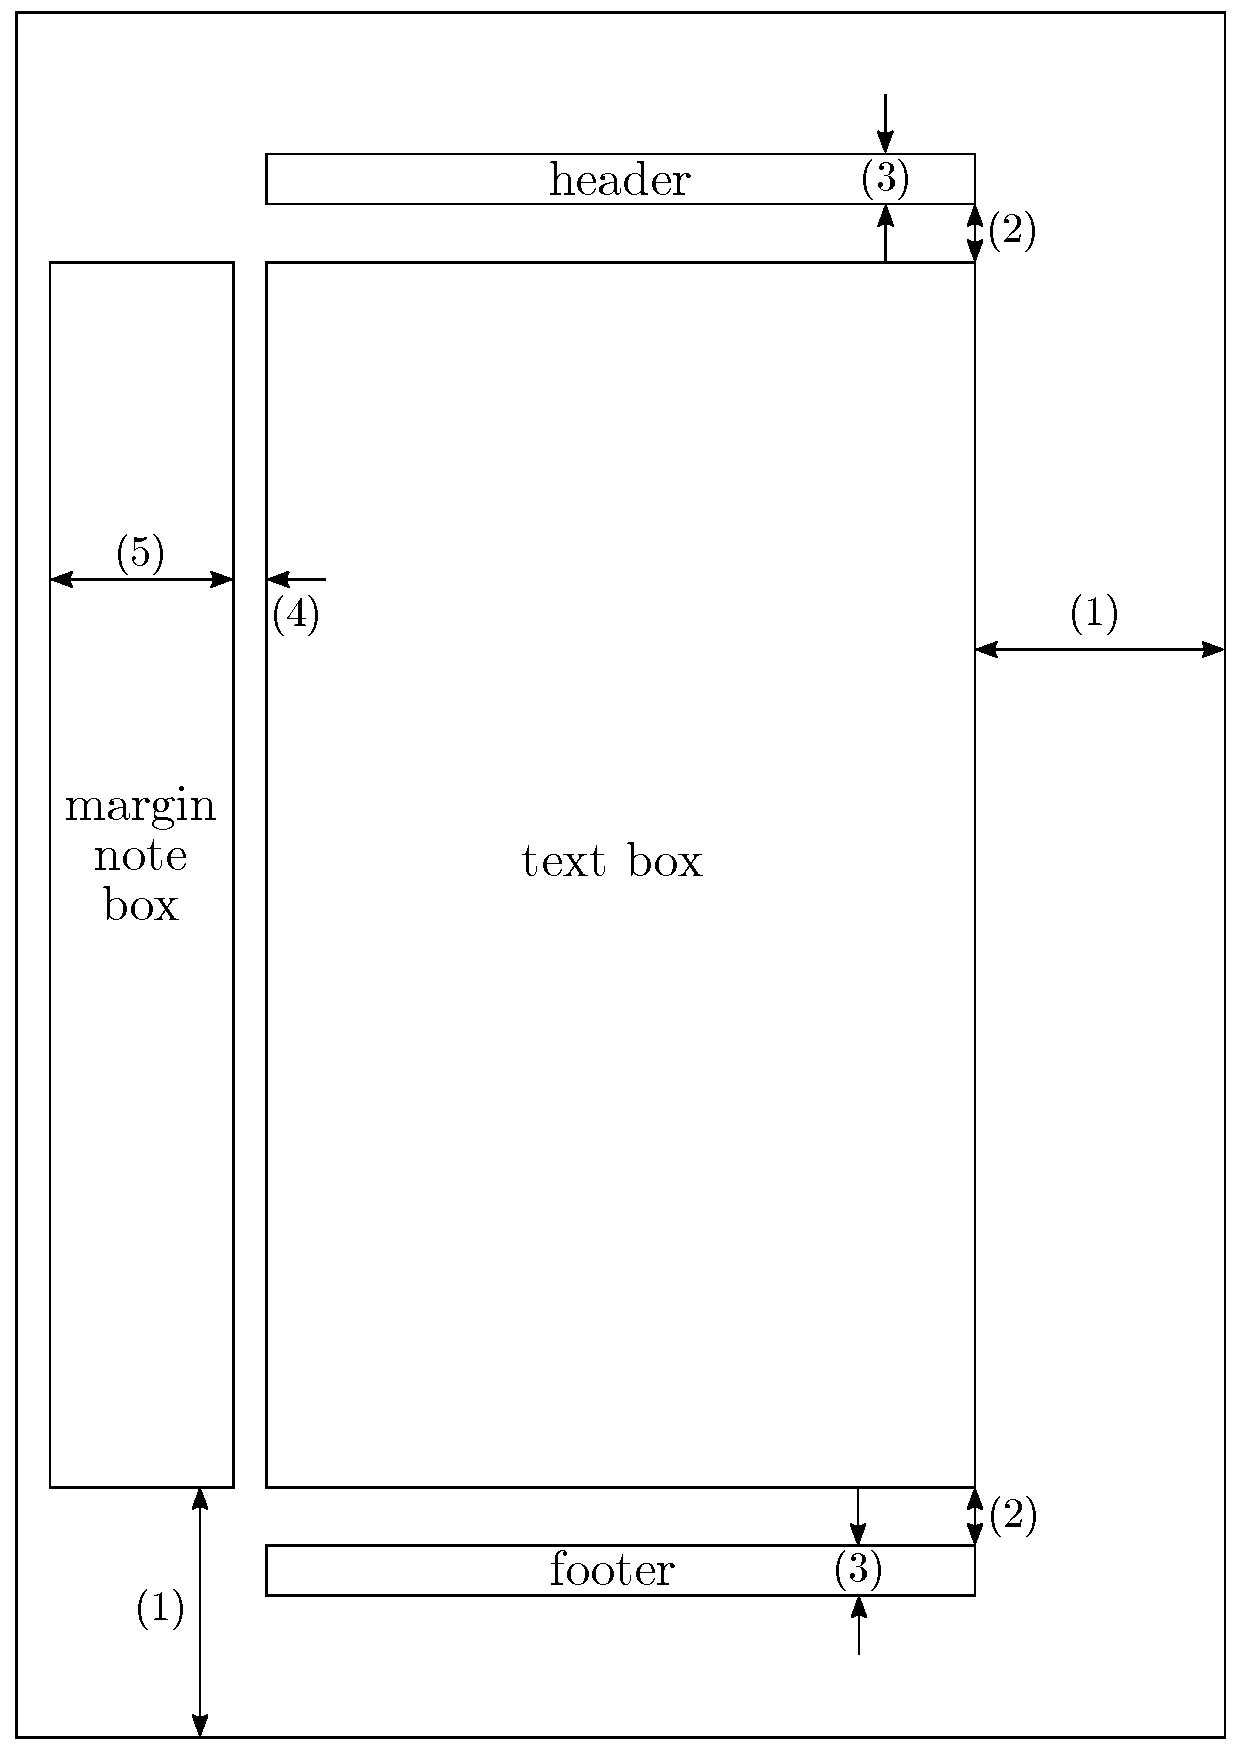
\includegraphics[scale=0.35]{pgdim.pdf}
    \end{center}
    \caption[Document page layout dimensions]{
        A page consists of four major fields -- the text, margin note, header, and footer -- as shown here.
        The main document text goes into the text box.
        Margin notes go into the margin note box, which can be on either the left, or right side of the page, depending on whether the page itself is a left hand side, or right hand side page.
        Page headers and footers are also allocated dedicated spaces on the page.
        The dimensions (1) to (5) that control the page layout are defined in Section \ref{sec:Page dimensions}.
    }
    \label{fig:Document page layout dimensions}
\end{figure}

\begin{listing}

\item   {\ttfamily\textbackslash @pgdim@textmargin}

        Space between page borders and text box borders.
        Dimension (1) in Figure \ref{fig:Document page layout dimensions}.

\item   {\ttfamily\textbackslash @pgdim@headerseparation}

        Separation between text box and header/footer box borders.
        Dimension (2) in Figure \ref{fig:Document page layout dimensions}.

\item   {\ttfamily\textbackslash @pgdim@headerheight}

        Height of header, and footer boxes.
        Dimension (3) in Figure \ref{fig:Document page layout dimensions}.

\item   {\ttfamily\textbackslash @pgdim@marginnoteseparation}

        Separation between text box and margin note box borders.
        Dimension (4) in Figure \ref{fig:Document page layout dimensions}.

\item   {\ttfamily\textbackslash @pgdim@marginnotewidth}

        Width of margin note box.
        Dimension (5) in Figure \ref{fig:Document page layout dimensions}.

\end{listing}

\section{Page decorations}\label{sec:Page decorations}

Macro name prefix: {\ttfamily\textbackslash @pgdec@}\\
Lines: 67 -- 74

\begin{listing}

\item   {\ttfamily\textbackslash @pgdec@leftheader}

        Command to generate the left hand side page header.

\item   {\ttfamily\textbackslash @pgdec@rightheader}

        Command to generate the right hand side page header.

\item   {\ttfamily\textbackslash @pgdec@leftfooter}

        Command to generate the left hand side page footer.

\item   {\ttfamily\textbackslash @pgdec@rightfooter}

        Command to generate the right hand side page footer.

\end{listing}

The control sequences {\ttfamily\textbackslash leftmark} and {\ttfamily\textbackslash rightmark} are often used within the definitions of the above macros.
These are page markings whose values are set by the {\ttfamily\textbackslash markboth} and {\ttfamily\textbackslash markright} commands.
The command {\ttfamily\textbackslash markboth\{<lmark>\}\{<rmark>\}} sets the value of {\ttfamily\textbackslash leftmark} to {\ttfamily<lmark>} and that of {\ttfamily\textbackslash rightmark} to {\ttfamily<rmark>}.
In the default version of {\ttfamily thesis.clo}, these commands are invoked by the {\ttfamily\textbackslash chapter} command (see Section \ref{sec:Document structure}) so that {\ttfamily\textbackslash leftmark} and {\ttfamily\textbackslash rightmark} indicate the current chapter heading.
Also, the values of {\ttfamily\textbackslash leftmark} and {\ttfamily\textbackslash rightmark} are used within the page headers.
This is the mechanism by which the {\ttfamily\textbackslash chapter} command updates the page headers.

\section{Document structure}\label{sec:Document structure}

Macro name prefix: {\ttfamily\textbackslash @docstruc@}\\
Lines: 75 -- 169

In the following listing, every instance of {\ttfamily<struc>} must be replaced by {\ttfamily chapter}, {\ttfamily section}, {\ttfamily subsection}, or {\ttfamily subsubsection}.

\begin{listing}

\item   {\ttfamily\textbackslash @docstruc@<struc>numberlesstocskip}

        Vertical space added to the table of contents whenever {\ttfamily\textbackslash<struc>} is executed to create an unnumbered {\ttfamily<struc>}.

\item   {\ttfamily\textbackslash @docstruc@<struc>numberedtocskip}

        Vertical space added to the table of contents whenever {\ttfamily\textbackslash<struc>} is executed to create a numbered {\ttfamily<struc>}.

\item   {\ttfamily\textbackslash @docstruc@<struc>numberlesslofskip}

        Vertical space added to the list of figures whenever {\ttfamily\textbackslash<struc>} is executed to create an unnumbered {\ttfamily<struc>}.

\item   {\ttfamily\textbackslash @docstruc@<struc>numberedlofskip}

        Vertical space added to the list of figures whenever {\ttfamily\textbackslash<struc>} is executed to create a numbered {\ttfamily<struc>}.

\item   {\ttfamily\textbackslash @docstruc@<struc>numberlesslotskip}

        Vertical space added to the list of tables whenever {\ttfamily\textbackslash<struc>} is executed to create an unnumbered {\ttfamily<struc>}.

\item   {\ttfamily\textbackslash @docstruc@<struc>numberedlotskip}

        Vertical space added to the list of tables whenever {\ttfamily\textbackslash<struc>} is executed to create a numbered {\ttfamily<struc>}.

\item   {\ttfamily\textbackslash @docstruc@make<struc>numberless\#1}

        Command to generate an unnumbered {\ttfamily<struc>} heading with {\ttfamily<struc>} name {\ttfamily\#1}.

\item   {\ttfamily\textbackslash @docstruc@make<struc>numbered\#1}

        Command to generate a numbered {\ttfamily<struc>} heading with {\ttfamily<struc>} name {\ttfamily\#1}.

\end{listing}

\section{Title page}\label{sec:Title page}

Macro name prefix: {\ttfamily\textbackslash @titlpg@}\\
Lines: 170 -- 205

\begin{listing}

\item   {\ttfamily\textbackslash @titlpg@create\#1\#2\#3\#4\#5\#6\#7\#8\#9}

        Command to create the title page with the 9 parameters {\ttfamily\#1} ... {\ttfamily\#9}.
        The arguments correspond to the values defined by the commands in Section \ref{sec:Title page parameters}.
        They are described below in the same order in which they are passed to {\ttfamily\textbackslash @titlpg@create}.

        \begin{enumeration}

        \item   Project title, as defined by the {\ttfamily\textbackslash title} command.

        \item   Purpose of submission, as defined by the {\ttfamily\textbackslash purpose} command.

        \item   Degree title, as defined by the {\ttfamily\textbackslash degree} command.

        \item   Academic field, as defined by the {\ttfamily\textbackslash subject} command.

        \item   Author name, as defined by the {\ttfamily\textbackslash author} command.

        \item   Author affiliation, as defined by the {\ttfamily\textbackslash authoraffil} command.

        \item   Project supervisor name, as defined by the {\ttfamily\textbackslash mentor} command.

        \item   Project supervisor affiliation, as defined by the {\ttfamily\textbackslash mentoraffil} command.

        \item   University logo creation command, as defined by the {\ttfamily\textbackslash logo} command.

        \end{enumeration}

\end{listing}

\section{Document contents}\label{sec:Document contents}

Macro name prefix: {\ttfamily\textbackslash @doccnts}\\
Lines: 206 -- 257

In the following listing, every instance of {\ttfamily<struc>} must be replaced by {\ttfamily chapter}, {\ttfamily section}, {\ttfamily subsection}, {\ttfamily subsubsection}, {\ttfamily figure}, or {\ttfamily table}.
Additionally, every instance of {\ttfamily<cnts>} must be replaced by ``table of contents'', ``list of figures'' or ``list of tables'' depending on what {\ttfamily<struc>} represents.

\begin{listing}

\item   {\ttfamily\textbackslash @doccnts@<struc>filler}

        Symbol to be repeatedly printed to fill up the space between a {\ttfamily<struc>} entry and the corresponding page number in the {\ttfamily<cnts>}.

\item   {\ttfamily\textbackslash @doccnts@<struc>indent}

        Amount of indentation added to a {\ttfamily<struc>} entry in the {\ttfamily<cnts>}.

\item   {\ttfamily\textbackslash @doccnts@<struc>numberwidth}

        Horizontal space within a {\ttfamily<struc>} entry, reserved for the {\ttfamily<struc>} number.
        This space is created even for unnumbered entries, but is left blank.

\item   {\ttfamily\textbackslash @doccnts@<struc>pagenumberwidth}

        Horizontal space within a {\ttfamily<struc>} entry, reserved for the page number.

\item   {\ttfamily\textbackslash @doccnts@<struc>fillerwidth}

        Space between successive filler symbols in a {\ttfamily<struc>} entry.

\item   {\ttfamily\textbackslash @doccnts@<struc>entryfont}

        Font used for the main text in a {\ttfamily<struc>} entry.

\item   {\ttfamily\textbackslash @doccnts@<struc>fillerfont}

        Font used for the filler in a {\ttfamily<struc>} entry.

\item   {\ttfamily\textbackslash @doccnts@<struc>pagenumberfont}

        Font used for the page number in a {\ttfamily<struc>} entry.

\end{listing}

\section{Figures and tables}\label{sec:Figures and tables}

Macro name prefix: {\ttfamily\textbackslash @figtab@}\\
Lines: 258 -- 271

\begin{listing}

\item   {\ttfamily\textbackslash @figtab@captionaboveskip}

        Vertical blank space above caption.

\item   {\ttfamily\textbackslash @figtab@captionbelowskip}

        Vertical blank space below caption.

\item   {\ttfamily\textbackslash @figtab@captionmargin}

        Horizontal blank space to the left and right of caption, added to the usual text margin.

\item   {\ttfamily\textbackslash @figtab@captionheadformat}

        Font used in the caption heading.

\item   {\ttfamily\textbackslash @figtab@captionbodyformat}

        Font used in the main caption body.

\item   {\ttfamily\textbackslash @figtab@figurelabeltext}

        Caption heading text for figures (full caption heading also contains the figure number).

\item   {\ttfamily\textbackslash @figtab@tablelabeltext}

        Caption heading text for tables (full caption heading also contains the table number).

\item   {\ttfamily\textbackslash @figtab@columnseparation}

        Horizontal separation between two consecutive columns in a table.

\item   {\ttfamily\textbackslash @figtab@rulewidth}

        Width of rules drawn in a table.

\item   {\ttfamily\textbackslash @figtab@doubleruleseparation}

        Separation between two rules placed next to each other to form a double rule.

\end{listing}

\clearpage

\section{Lists and enumerations}\label{sec:Lists and enumerations}

Macro name prefix: {\ttfamily\textbackslash @lstenum@}\\
Lines: 272 -- 291

\begin{figure}
    \begin{center}
        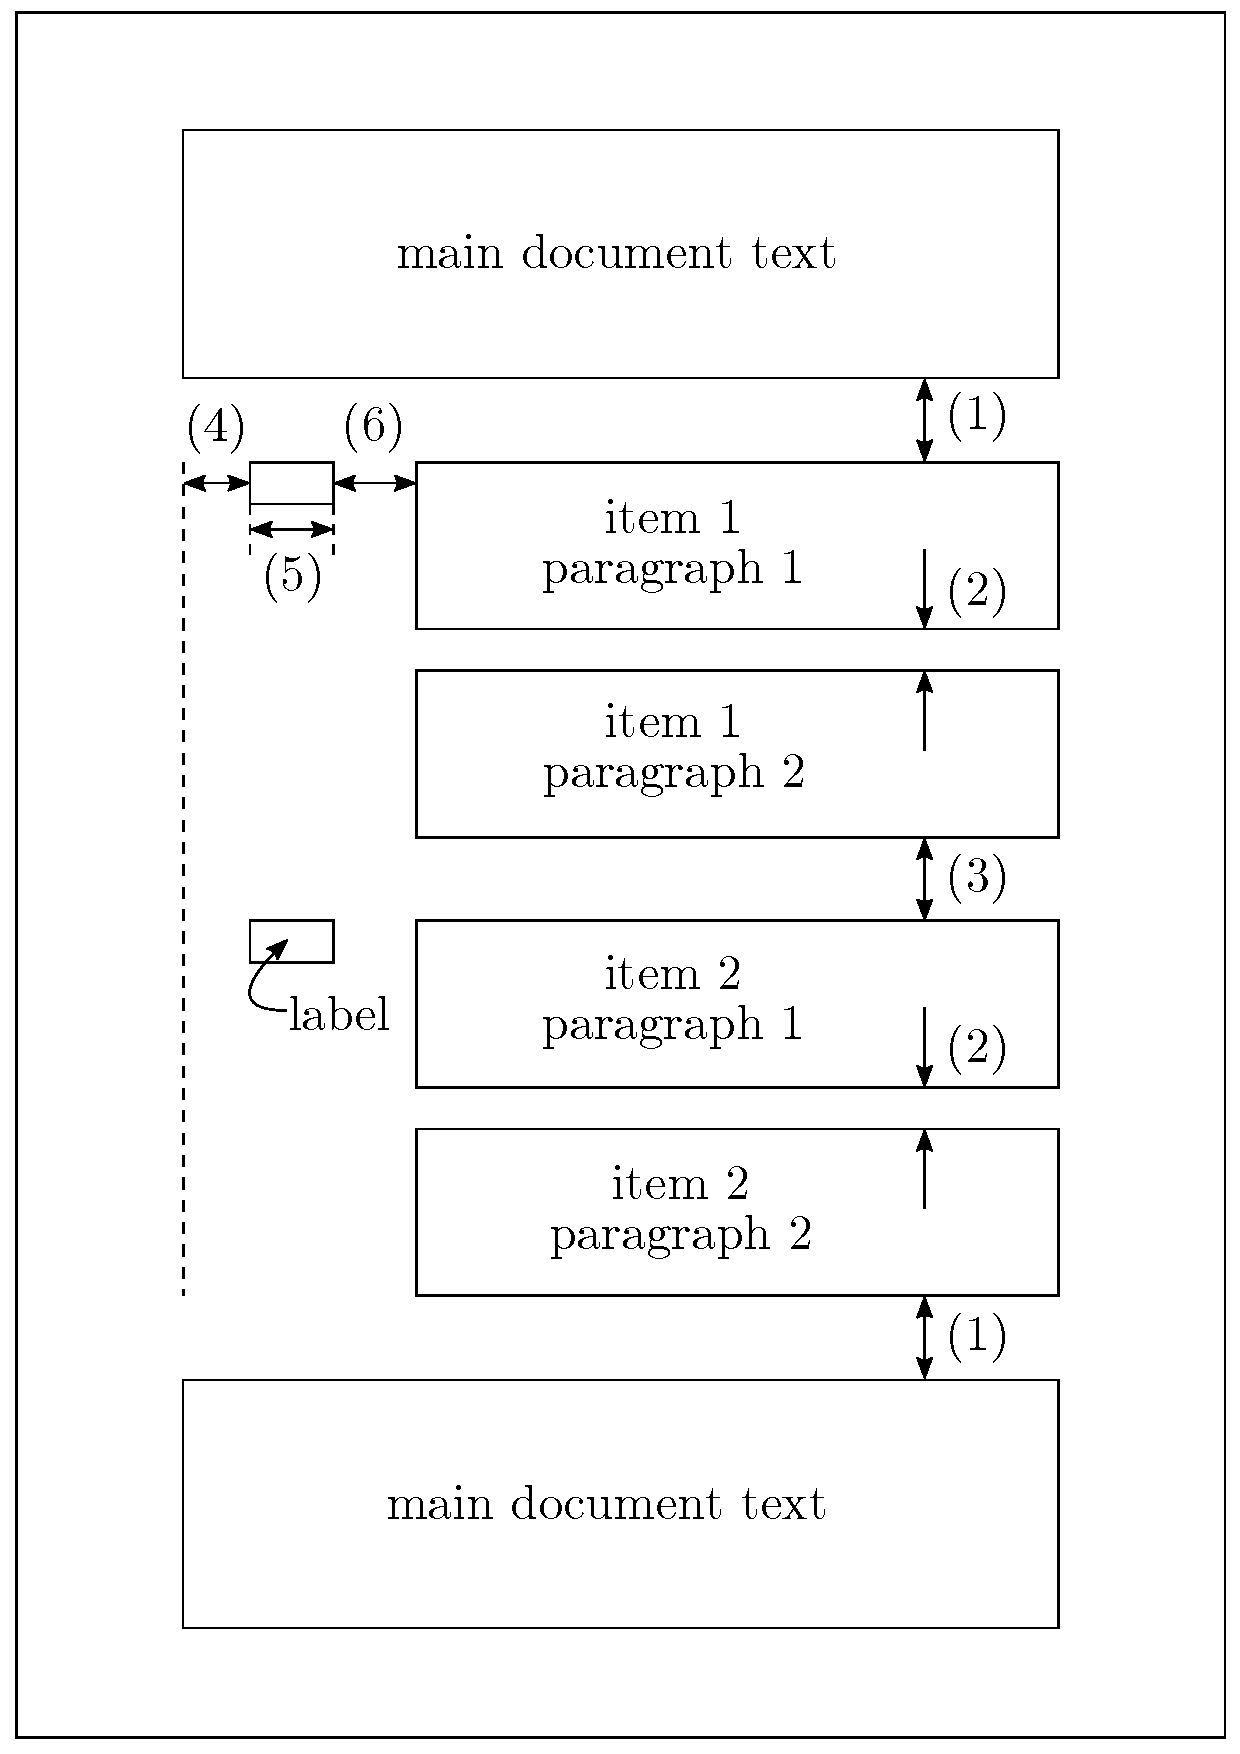
\includegraphics[scale=0.35]{lstenum.pdf}
    \end{center}
    \caption[List layout dimensions]{
        Each list consists of multiple entries, called items.
        Every item has a label which has a box reserved for itself.
        The textual content of the item is formatted into paragraphs as shown.
        The dimensions(1) to (6) that control the list layout are described in Section \ref{sec:Lists and enumerations}.
    }
    \label{fig:List layout dimensions}
\end{figure}

\begin{listing}

\item   {\ttfamily\textbackslash @lstenum@labelmargin}

        Space between left text margin and label box border.
        Dimension (4) in Figure \ref{fig:List layout dimensions}.

\item   {\ttfamily\textbackslash @lstenum@labelwidth}

        Width of box reserved for label.
        Dimension (5) in Figure \ref{fig:List layout dimensions}.

\item   {\ttfamily\textbackslash @lstenum@labelseparation}

        Space between label box and item paragraph box borders.
        Dimension (6) in Figure \ref{fig:List layout dimensions}.

\item   {\ttfamily\textbackslash @lstenum@itemseparation}

        Space between two consecutive items, in addition to item paragraph separation.
        Dimension (3) minus dimension (2) in Figure \ref{fig:List layout dimensions}.

\item   {\ttfamily\textbackslash @lstenum@paragraphseparation}

        Space between two paragraphs within a single item.
        Dimension (2) in Figure \ref{fig:List layout dimensions}.

\item   {\ttfamily\textbackslash @lstenum@aboveseparation}

        Space left above and below the list structure in addition to the default paragraph spacing in the main document text.
        Dimension (1) minus {\ttfamily\textbackslash parskip} in Figure \ref{fig:List layout dimensions}.

\item   {\ttfamily\textbackslash @lstenum@listinglabeli}

        Symbol used as label for top-level items in {\ttfamily listing} environments.

\item   {\ttfamily\textbackslash @lstenum@listinglabelii}

        Symbol used as label for items at nesting depth of 2, in {\ttfamily listing} environments.

\item   {\ttfamily\textbackslash @lstenum@listinglabeliii}

        Symbol used as label for items at nesting depth of 3, in {\ttfamily listing} environments.

\item   {\ttfamily\textbackslash @lstenum@listinglabeliv}

        Symbol used as label for items at nesting depth of 4, in {\ttfamily listing} environments.

\item   {\ttfamily\textbackslash @lstenum@enumerationlabeli}

        Label format for top-level items in {\ttfamily enumeration} environments.

\item   {\ttfamily\textbackslash @lstenum@enumerationlabelii}

        Label format for items at nesting depth of 2, in {\ttfamily enumeration} environments.

\item   {\ttfamily\textbackslash @lstenum@enumerationlabeliii}

        Label format for items at nesting depth of 3, in {\ttfamily enumeration} environments.

\item   {\ttfamily\textbackslash @lstenum@enumerationlabeliv}

        Label format for items at nesting depth of 4, in {\ttfamily enumeration} environments.

\end{listing}

\section{Technical blocks}\label{sec:Technical blocks}

Macro name prefix: {\ttfamily\textbackslash @techblk@}\\
Lines: 292 -- 298

\begin{listing}

\item   {\ttfamily\textbackslash @techblk@headfont}

        Font used in block heading.

\item   {\ttfamily\textbackslash @techblk@emphasizedbodyfont}

        Font used in main body of blocks with the {\ttfamily emph} option enabled.

\item   {\ttfamily\textbackslash @techblk@normalbodyfont}

        Font used in main body of blocks with the {\ttfamily noemph} option enabled.

\item   {\ttfamily\textbackslash @techblk@terminationmark}

        The Q.E.D.\ symbol to use for blocks with the {\ttfamily term} option enabled.

\end{listing}

\appendix

\chapter{Font selection}\label{ap:Font selection}

Old font selection commands such as {\ttfamily\textbackslash textbf} or {\ttfamily\textbackslash textit} are not supported in the {\ttfamily thesis} class.
Only the newer font selection commands should be used in the source text.
The following sections enlist the supported font selection commands for both, textual, and mathematical modes.

\section{Textual fonts}\label{sec:Textual fonts}

Fonts in textual mode are defined by four attributes -- size, family, series, and shape.
The value of each attribute can be specified by a corresponding set of commands.
Sections \ref{subsec:Font size commands} to \ref{subsec:Font shape commands} list out the commands for each attribute.

\subsection{Font size commands}\label{subsec:Font size commands}

The following are the font size commands in decreasing order of size.

\begin{listing}

\item   {\ttfamily\textbackslash Huge}

\item   {\ttfamily\textbackslash huge}

\item   {\ttfamily\textbackslash LARGE}

\item   {\ttfamily\textbackslash Large}

\item   {\ttfamily\textbackslash large}

\item   {\ttfamily\textbackslash normalsize}

\item   {\ttfamily\textbackslash small}

\item   {\ttfamily\textbackslash footnotesize}

\item   {\ttfamily\textbackslash scriptsize}

\item   {\ttfamily\textbackslash tiny}

\end{listing}

\clearpage

\subsection{Font family commands}\label{subsec:Font family commands}

\begin{listing}

\item   {\ttfamily\textbackslash rmfamily}

        Roman font family.

\item   {\ttfamily\textbackslash sffamily}

        Sans serif font family.

\item   {\ttfamily\textbackslash ttfamily}

        Typewriter text font family.

\end{listing}

\subsection{Font series commands}\label{subsec:Font series commands}

\begin{listing}

\item   {\ttfamily\textbackslash mdseries}

        Medium weight font (default appearance).

\item   {\ttfamily\textbackslash bfseries}

        Boldface font.

\end{listing}

\subsection{Font shape commands}\label{subsec:Font shape commands}

\begin{listing}

\item   {\ttfamily\textbackslash upshape}

        Upright font shape.

\item   {\ttfamily\textbackslash itshape}

        Italic font shape.

\item   {\ttfamily\textbackslash slshape}

        Slanted font shape.

\item   {\ttfamily\textbackslash scshape}

        Small-caps font shape.

\end{listing}

\section{Mathematical fonts}\label{sec:Mathematical fonts}

In mathematical mode, the following font selection commands must be used instead of those presented in Section \ref{sec:Textual fonts}.

\begin{listing}

\item   {\ttfamily\textbackslash mathrm}

        Roman font.

\item   {\ttfamily\textbackslash mathit}

        Italic font.

\item   {\ttfamily\textbackslash mathbf}

        Boldface font.

\item   {\ttfamily\textbackslash mathsf}

        Sans serif font.

\item   {\ttfamily\textbackslash mathtt}

        Typewriter font.

\item   {\ttfamily\textbackslash mathcal}

        Calligraphic font (use only for upper case alphabets).

\end{listing}

\chapter{Automatic hyperlinks}\label{ap:Automatic hyperlinks}

All references created with the {\ttfamily\textbackslash ref} and {\ttfamily\textbackslash eqref} commands, citation marks created using {\ttfamily\textbackslash cite} (see Appendix \ref{ap:Creating the bibliography}), entries in the table of contents, etc.\ can automatically be converted into hyperlinks.
In order to do this, simply include the {\ttfamily hyperref} package in the preamble.

{\ttfamily\textbackslash usepackage\{hyperref\}}

The appearance of the hyperlinks in the document can be controlled using the {\ttfamily\textbackslash hypersetup} command.
For example, custom colours can be specified for different types of hyperlinks in the following way.

{\ttfamily
    \textbackslash usepackage\{xcolors\}\linebreak
    \textbackslash usepackage\{hyperref\}\linebreak
    \linebreak
    \textbackslash definecolor\{hreflink\}\{RGB\}\{150,75,0\}\linebreak
    \textbackslash definecolor\{hrefcite\}\{RGB\}\{200,0,200\}\linebreak
    \textbackslash definecolor\{hrefurl\}\{RGB\}\{0,50,200\}\linebreak
    \linebreak
    \textbackslash hypersetup\{\linebreak
        \null\quad colorlinks = true,\linebreak
        \null\quad linkcolor = hreflink,\linebreak
        \null\quad citecolor = hrefcite,\linebreak
        \null\quad urlcolor = hrefurl\linebreak
    \}
}

In this example, RGB colours are defined using the {\ttfamily\textbackslash definecolor} command from the package {\ttfamily xcolor}.
The newly defined colour names are then used in the {\ttfamily\textbackslash hypersetup} command.

Detailed information about {\ttfamily\textbackslash hypersetup} can be found in the \href{https://ftp.agdsn.de/pub/mirrors/latex/dante/macros/latex/contrib/hyperref/doc/manual.pdf}{official documentation} of the {\ttfamily hyperref} package.

\chapter{Creating the bibliography}\label{ap:Creating the bibliography}

The bibliography can be created in the usual way, using {\scshape Bib\TeX}.
The {\ttfamily biblatex} package must be imported, and a {\ttfamily*.bib} file containing {\scshape Bib\TeX} entries for each cited reference should be created.
This file should then be added as a bibliography resource.
For example, if {\ttfamily thesis.bib} is the bibliography resource file, then the following should be put into the preamble code.

{\ttfamily
    \textbackslash usepackage[backend=biber]\{biblatex\}\linebreak
    \textbackslash addbibresource\{thesis.bib\}
}

The {\ttfamily\textbackslash cite} command can be used to cite any reference defined in the {\ttfamily*.bib} file.
Donald Knuth's {\itshape The \TeX book} \cite{knuth1984} was cited in this document using this command.

The command {\ttfamily\textbackslash nocite} can be used instead of {\ttfamily\textbackslash cite} if an entry should be added to the bibliography, without creating a citation mark in the text.
For example, Matplotlib has been cited in this document using {\ttfamily\textbackslash nocite}.

Detailed information on using the {\ttfamily biblatex} package can be found in its \href{https://ctan.net/macros/latex/contrib/biblatex/doc/biblatex.pdf}{official documentation}.

\back

\chapter{Bibliography}

\nocite{hunter2007}

\printbibliography[heading=none]

\end{document}
